% flashcards-title: Equivalent one-half and two-fourths strips
% flashcards-desc: Two equal-length bars are shaded to the halfway point; one is divided into halves and the other into fourths.
\documentclass[dvisvgm,tikz,border=8pt]{standalone}
\usetikzlibrary{arrows.meta,patterns}

\definecolor{qraNavy}{HTML}{17324D}
\definecolor{qraBlue}{HTML}{2B6CB0}
\definecolor{qraGold}{HTML}{B7791F}
\definecolor{qraPale}{HTML}{EAF2F8}
\definecolor{qraGray}{HTML}{5C6773}

\tikzset{
  qra axis/.style={draw=qraNavy, line width=1.2pt},
  qra tick/.style={draw=qraNavy, line width=1pt},
  qra guide/.style={draw=qraGray, densely dashed, line width=0.8pt},
  qra counter/.style={circle, draw=qraNavy, fill=qraPale, line width=0.9pt, minimum size=7mm, inner sep=0pt},
  qra label/.style={font=\sffamily\bfseries, text=qraNavy},
  qra small label/.style={font=\sffamily, text=qraNavy},
}

\begin{document}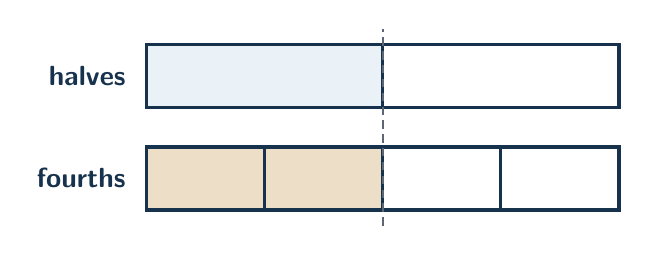
\begin{tikzpicture}[x=1cm,y=1cm]
\fill[qraPale](0,1.3)rectangle(3,2.1);\draw[qra axis](0,1.3)rectangle(6,2.1);\draw[qra tick](3,1.3)--(3,2.1);\node[qra label,left=4pt]at(0,1.7){halves};
\fill[qraGold!25](0,0)rectangle(3,.8);\draw[qra axis](0,0)rectangle(6,.8);\foreach \x in {1.5,3,4.5}{\draw[qra tick](\x,0)--(\x,.8);}\node[qra label,left=4pt]at(0,.4){fourths};
\draw[qra guide](3,-.2)--(3,2.3);
\end{tikzpicture}\end{document}
